\documentclass[a4paper,12pt]{article}
\usepackage{amsmath}
\usepackage{amssymb,amsthm,graphicx}
\usepackage{titlesec}
\usepackage{textcomp}
\usepackage{enumitem}
\usepackage{color}
\usepackage{epsfig}
\usepackage{graphics}
\usepackage{pdfpages}
\usepackage{subcaption}
\usepackage[font=small]{caption}
\usepackage[hang,flushmargin]{footmisc} 
\usepackage{float}
\usepackage{rotating,tabularx}
\usepackage{booktabs}
\usepackage[mathscr]{euscript}
\usepackage{natbib}
\usepackage{setspace}
\usepackage{mathrsfs}
\usepackage[official]{eurosym}
\usepackage[left=2.8cm,right=2.8cm,bottom=2.8cm,top=2.5cm]{geometry}

\setcounter{secnumdepth}{4}
\renewcommand{\baselinestretch}{1.2}


% General

\newcommand{\reals}{\mathbb{R}}
\newcommand{\integers}{\mathbb{Z}}
\newcommand{\naturals}{\mathbb{N}}

\newcommand{\pr}{\mathbb{P}}        % probability
\newcommand{\ex}{\mathbb{E}}        % expectation
\newcommand{\var}{\textnormal{Var}} % variance
\newcommand{\cov}{\textnormal{Cov}} % covariance

\newcommand{\law}{\mathcal{L}} % law of X
\newcommand{\normal}{N}        % normal distribution 

\newcommand{\argmax}{\textnormal{argmax}}
\newcommand{\argmin}{\textnormal{argmin}}

\newcommand{\ind}{\mathbbm{1}} % indicator function
\newcommand{\kernel}{K} % kernel function
\newcommand{\wght}{W} % kernel weight
\newcommand{\thres}{\pi} % threshold parameter


% Convergence

\newcommand{\convd}{\stackrel{d}{\longrightarrow}}              % convergence in distribution
\newcommand{\convp}{\stackrel{P}{\longrightarrow}}              % convergence in probability
\newcommand{\convas}{\stackrel{\textrm{a.s.}}{\longrightarrow}} % convergence almost surely
\newcommand{\convw}{\rightsquigarrow}                           % weak convergence


% Theorem-like declarations

\theoremstyle{plain}

\newtheorem{theorem}{Theorem}[section]
\newtheorem{prop}[theorem]{Proposition}
\newtheorem{lemma}[theorem]{Lemma}
\newtheorem{corollary}[theorem]{Corollary}
\newtheorem*{theo}{Theorem}
\newtheorem{propA}{Proposition}[section]
\newtheorem{lemmaA}[propA]{Lemma}
\newtheorem{definition}{Definition}[section]
\newtheorem{remark}{Remark}[section]
\renewcommand{\thelemmaA}{A.\arabic{lemmaA}}
\renewcommand{\thepropA}{A.\arabic{propA}}
\newtheorem*{algo}{Clustering Algorithm}


% Theorem numbering to the left

\makeatletter
\newcommand{\lefteqno}{\let\veqno\@@leqno}
\makeatother


% Heading

\newcommand{\heading}[2]
{  \setcounter{page}{1}
   \begin{center}

   \phantom{Distance to upper boundary}
   \vspace{0.5cm}

   {\LARGE \textbf{#1}}
   \vspace{0.4cm}
 
   {\LARGE \textbf{#2}}
   \end{center}
}


% Authors

\newcommand{\authors}[4]
{  \parindent0pt
   \begin{center}
      \begin{minipage}[c][2cm][c]{5cm}
      \begin{center} 
      {\large #1} 
      \vspace{0.05cm}
      
      #2 
      \end{center}
      \end{minipage}
      \begin{minipage}[c][2cm][c]{5cm}
      \begin{center} 
      {\large #3}
      \vspace{0.05cm}

      #4 
      \end{center}
      \end{minipage}
   \end{center}
}

%\newcommand{\authors}[2]
%{  \parindent0pt
%   \begin{center}
%   {\large #1} 
%   \vspace{0.1cm}
%      
%   #2 
%   \end{center}  
%}


% Version

\newcommand{\version}[1]
{  \begin{center}
   {\large #1}
   \end{center}
   \vspace{3pt}
} 










\begin{document}

 

\noindent {\Large \bf Answer to the Referee Report I} 
\vspace{0.25cm}

\begin{itemize}
\item A consistency result of Proposition 3.3.

I believe that the following type of result can be obtained: $\Pr (E^l_T) \to 1$. Theorem 3.1 is for testing purpose. In certain application one might be interested in such consistency result. Basically one needs to study the behavior of $q_T (\alpha)$ when $\alpha \to 0$.

\item Estimation of long run variance using autoregressive processes.

The authors considered estimating $\sigma^2$ using AR processes. A limitation is that the order $p$ is fixed and finite. It appears that the latter limitation can be relaxed. For a stationary process $\varepsilon_t$ (not necessarily linear), one can fit an AR process with large $p$
$$ \varepsilon_t = \sum_{j=1}^p a_j \varepsilon_{t-j} + \eta_t,$$
properties of fitted $\widehat{a}_1, \ldots, \widehat{a}_p$ can be obtained from the results in the following papers
\begin{itemize}
\item W. B. Wu and Mohsen Pourahmadi (2009): Banding Sample Covariance Matrices of Stationary Processes, Statistica Sinica 19 1755-1768.
\item H. Xiao and W. B. Wu (2012). Covariance Matrix Estimation for Stationary Time Series. Annals of Statistics, Volume 40, Number 1 (2012), 466-493.
\end{itemize}
A similar version of the authors estimate (4.14) can be used. Rate of convergence (cf. Proposition 4.1) can be derived with rate $T^{-1/2}$ therein possibly replaced by a larger term of the form $T^{-c}$ with $c < 1/2$.

\item Real data application.

The authors analyzed the yearly mean Central England temperature data. It will be interesting to apply their approach to the global temperature data. In the paper ``Isotonic regression: another look at the change point problem. Biometrika, 88, 793-804, 2001'', an increasing trend function is fitted. It will be important to know which period the sequence in increasing/decreasing.

\item Simulation Study

In the simulation study the authors considered AR(1) processes with relatively weaker dependence: $a_1 \in \{-0.5, -0.25, 0.25, 0.5\}$. One should consider the stronger positive/negative dependence case with $a = \pm 0.9$ (say). How does the strength of dependence affect the performance of the procedure?

\end{itemize}


\newpage
\noindent {\Large \bf Answer to the Referee Report II} 
\vspace{0.25cm}

\begin{enumerate}
\item Section 3.2: The authors recommend computing the quantiles for the independent Gaussian case by simulation. This suggestion is already in the original SiZer paper (Chaudhuri and Marron, 1999). However in the late 1990s computing power was not sufficient to make this suggestion feasible. This led to the use of approximation such as in Hannig and Marron (2006). I would like to ask how does the simulation based quantile compare to the approximation in Hannig and Marron (2006). 

-- Compare multiscale test with and without additive correction terms $\lambda(h)$ by ``parallel coordinate plots'' as in Figure 5 of Hannig \& Marron (2006). 

\item Page 12, line 15: What is random here? After a spending some time I believe that it is the $\Pi_T$ but on first reading I thought $E_T$s are non-random. Please explain these various objects better.
\item Page 18, line 52: Please remove the speculative statements about what can be shown unless you actually show it in this paper.

\item Section 4.1: This section does not contain any truly new material and should be removed.

\item Section 5.2: I understand that you are doing comparisons to SiZer out of the box. However, some of the comparison might not be quite fair. SiZer is adjusting multiplicity ”row-wise” while the proposed method is attempting a global multiple control. What would happen if your $G_T$ only focused on one scale?

What's done (here $\alpha$ is always taken to be $0.05$):
\begin{itemize}
\item For each setting, each sample size, and each bandwidth row we report the percentage of realizations of the data in which there were some red or blue pixels in that row. The reports are given in ``parallel coordinate plots'' as in Figure 5 of \cite*{HannigMarron2006}. Each plot has the results of SiZer, the results of our global method and the results of our rowwise method respectively. The settings are as follows:
\begin{enumerate}
\item Under the null for $a_1 = -0.25, 0, 0.25$ and sample size $T = 250$.
\item Under the alternative for $a_1 = -0.25, 0$ and sample size $T = 250$. The trend function is linear increasing on the whole interval with the slope $\beta = 1.25$. 
\item Under the alternative for $a_1 = 0.25$ and sample size $T = 250$. The trend function is linear increasing on the whole interval with the slope $\beta = 2.25$. 
\end{enumerate}
\item Representative SiZer maps (for SiZer, our global method and our rowwise method) for simulated data from the null distribution for $a_1 = -0.25, 0, 0.25$. Sample size is $T = 250$. $1,000$ such SiZer maps were simulated for each setting and the population of them was ordered in terms of number of pixels that flag significant structure by being red or blue. For each setting and for each method we show 500th of these maps (essentially the median of the population), the 750th (the third quartile), the 850th and the 950th member of the ordered population.
\end{itemize}

\item Page 25, line 1-26: I do not quite understand this figure. Would it be possible to rather reproduce the colorful SiZer figures that show the results of the test at various scales and locations? Also you should use several different signals. I believe that a single relatively large bump is not sufficient test bed. A good collection of signals can be found in Donoho and Johnstone (1995). Also, would Hannig et al. (2013) be helpful in comparing the results?

What's done (here $\alpha$ is always taken to be $0.05$):
\begin{itemize}
\item Plots comparing SiZer maps under the null:
\begin{enumerate}
\item Plots comparing SiZer and global method and rowwise methods respectively for sample size is $T=250$. AR(1) parameters are $a_1 = -0.25, 0, 0.25$ and $\sigma_\eta^2 = 1$.
\end{enumerate}
\item Plots comparing SiZer maps under the alternative:
\begin{enumerate}
\item Plots comparing SiZer and global method and rowwise methods respectively for sine curve plus AR(1) noise (as in \cite*{ParkHannigKang2009}) for sample size $T=250$. AR(1) parameters are $a_1 = -0.25, 0, 0.25$ and $\sigma_\eta^2 = 1$.
\item Plots comparing SiZer and global method and rowwise methods respectively for blocks plus AR(1) noise (signal from \cite*{Donoho1995}, recentered and normalized as in \cite*{HannigMarron2006}) for sample size $T=250$. AR(1) parameters are $a_1 = -0.25, 0, 0.25$ and $\sigma_\eta^2 = 0.01$.
\item Plots comparing SiZer and global method and rowwise methods respectively for blocks plus AR(1) noise (signal from \cite*{Donoho1995}, recentered and normalized as in \cite*{HannigMarron2006}) for sample size $T=1000$. AR(1) parameters are $a_1 = -0.25, 0, 0.25$ and $\sigma_\eta^2 = 0.01$.
\end{enumerate}
\end{itemize}

Different signals: \\
-- Power results could be reported in terms of ability to find the jump points in the blocks example. 

\item Page 31, line 1-39: Can you plot the SiZer results on this data?
\end{enumerate}

\begin{figure}[t!]
\begin{subfigure}[b]{0.475\textwidth}
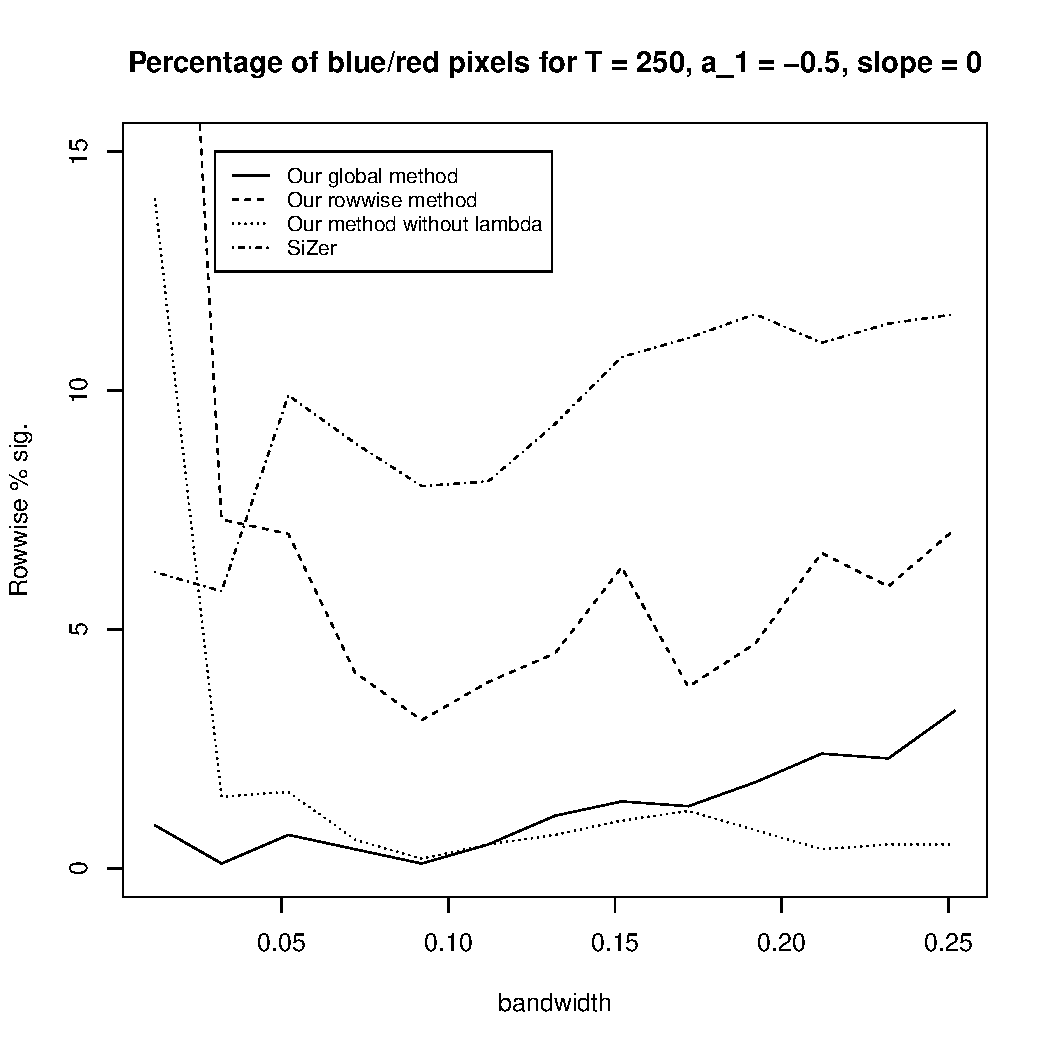
\includegraphics[width=\textwidth]{Plots/rowwise_sig_comparison_T_250_a1_-50_slope_0.pdf}
\caption{$a_1 = -0.5$, slope = $0$}
\end{subfigure}\hspace{0.25cm}
\begin{subfigure}[b]{0.475\textwidth}
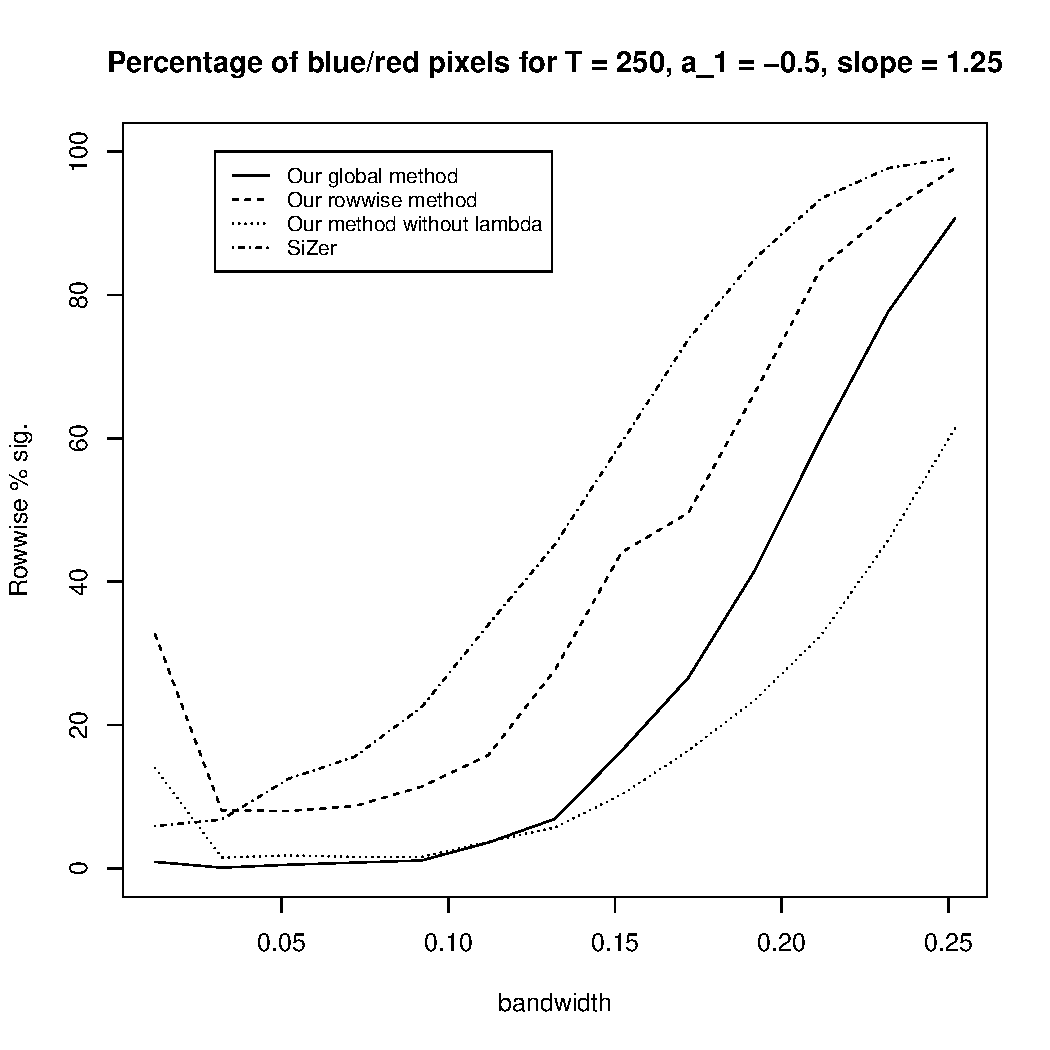
\includegraphics[width=\textwidth]{Plots/rowwise_sig_comparison_T_250_a1_-50_slope_125.pdf}
\caption{$a_1 = -0.5$, slope = $1,25$}
\end{subfigure}\\
\begin{subfigure}[b]{0.475\textwidth}
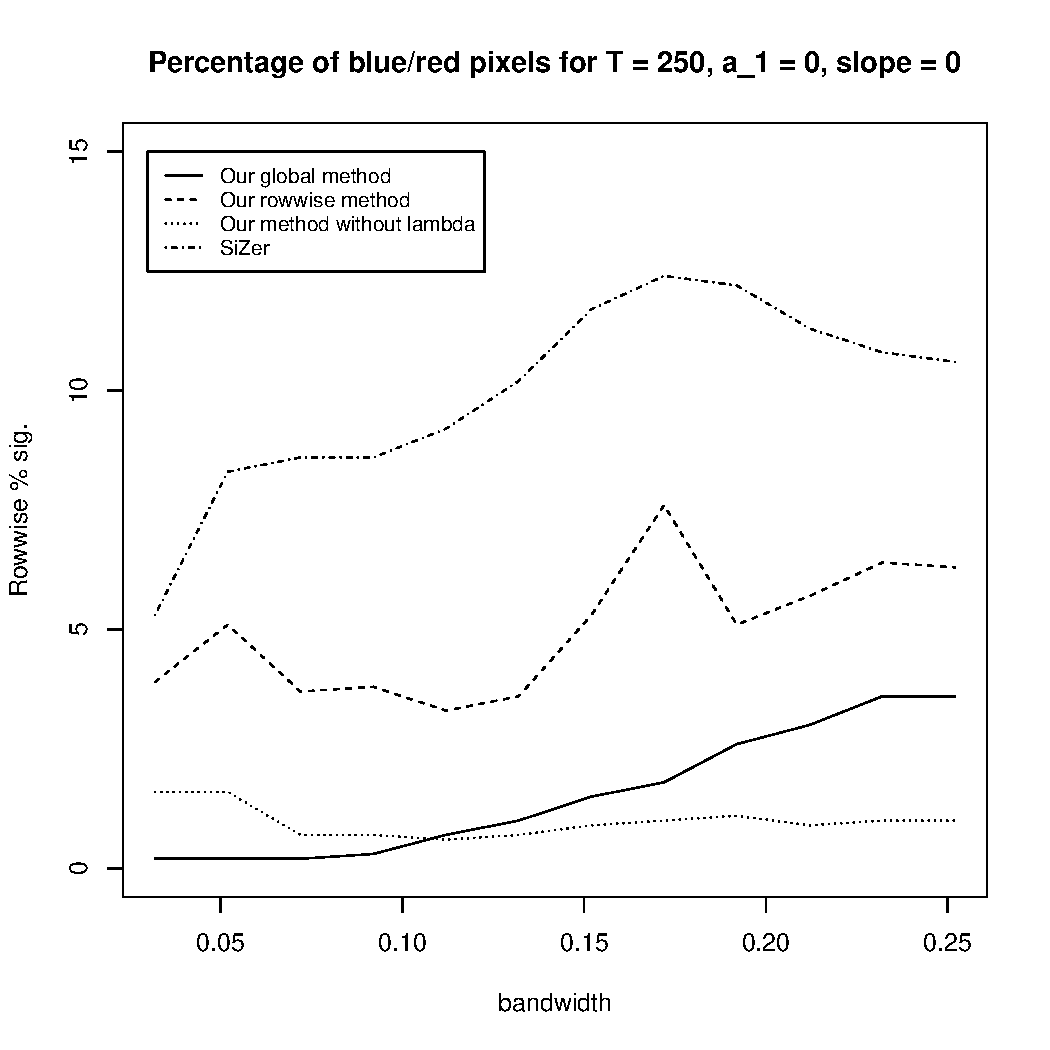
\includegraphics[width=\textwidth]{Plots/rowwise_sig_comparison_T_250_a1_0_slope_0.pdf}
\caption{$a_1 = 0$, slope = $0$}
\end{subfigure}\hspace{0.25cm}
\begin{subfigure}[b]{0.475\textwidth}
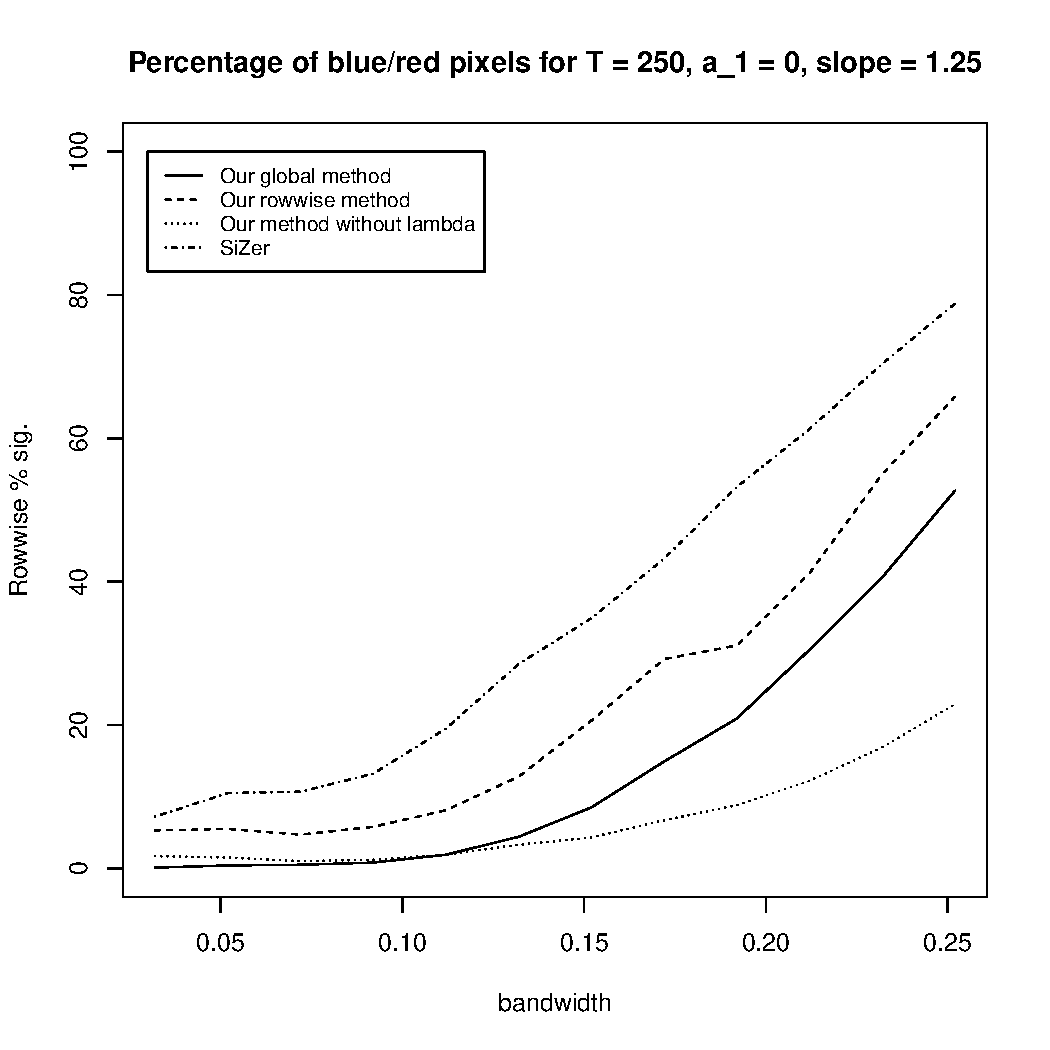
\includegraphics[width=\textwidth]{Plots/rowwise_sig_comparison_T_250_a1_0_slope_125.pdf}
\caption{$a_1 = 0$, slope = $1.25$}
\end{subfigure}\\
\begin{subfigure}[b]{0.475\textwidth}
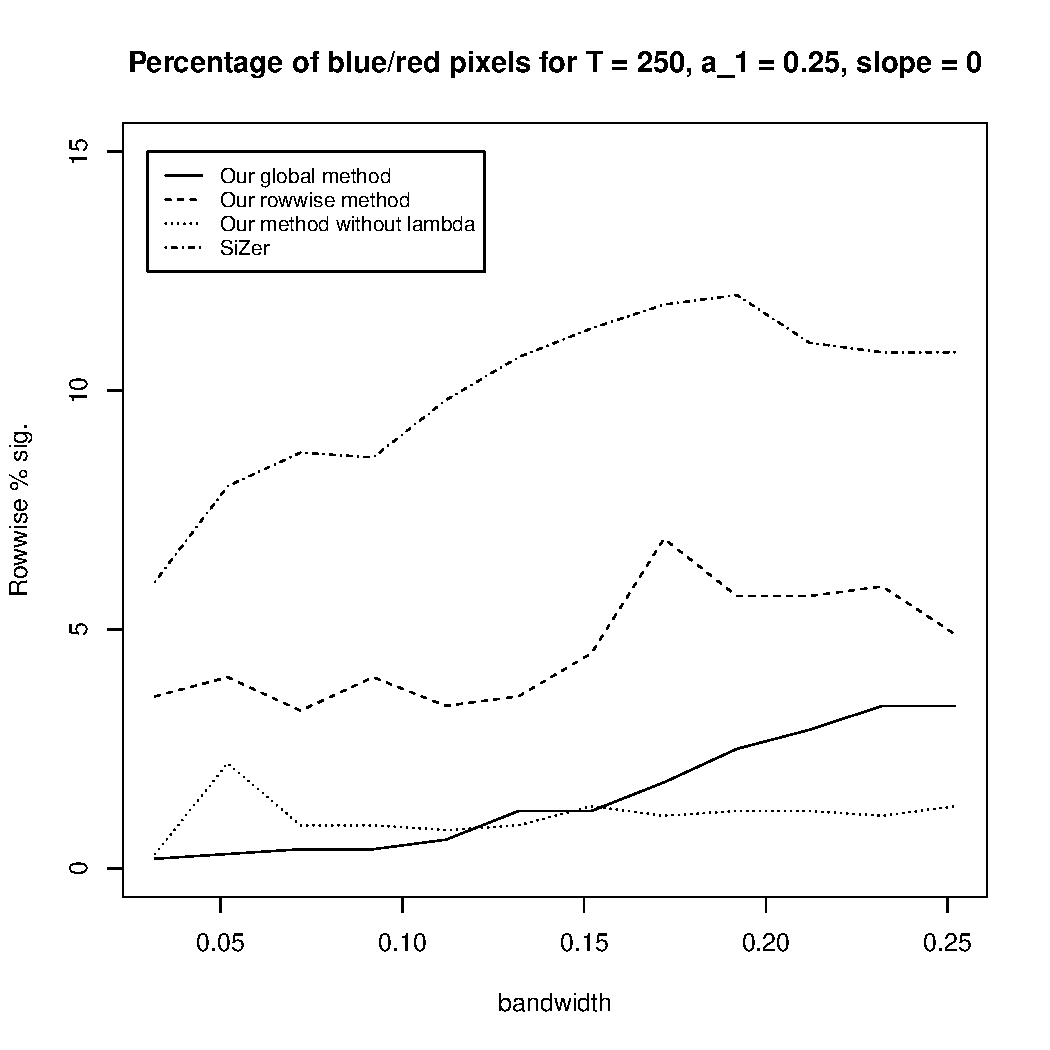
\includegraphics[width=\textwidth]{Plots/rowwise_sig_comparison_T_250_a1_25_slope_0.pdf}
\caption{$a_1 = 0.25$, slope = $0$}
\end{subfigure}\hspace{0.25cm}
\begin{subfigure}[b]{0.475\textwidth}
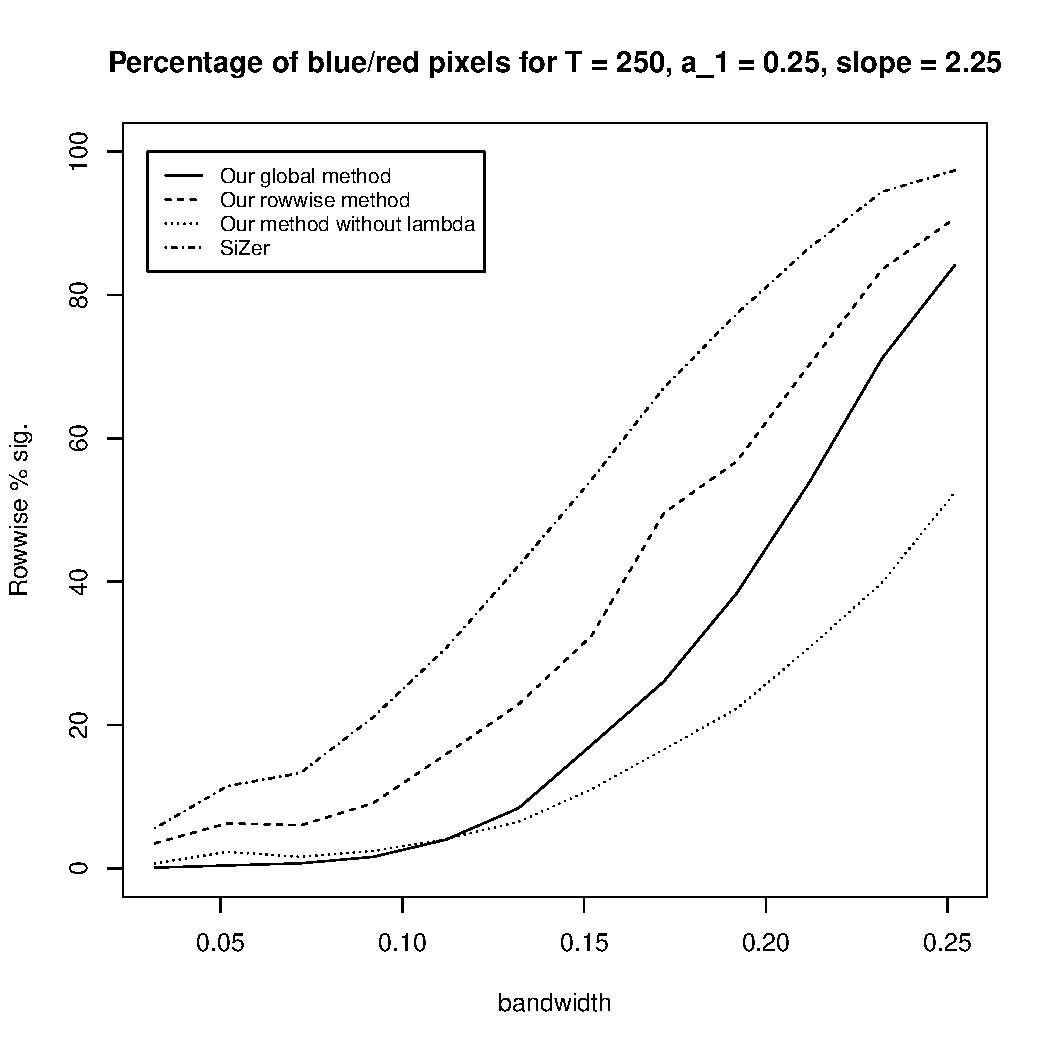
\includegraphics[width=\textwidth]{Plots/rowwise_sig_comparison_T_250_a1_25_slope_225.pdf}
\caption{$a_1 = 0.25$, slope = $2.25$}
\end{subfigure}
\caption{Parallel coordinate plots for $T = 250$ and different AR(1) parameters $a_1 = -0.5, 0, 0.25$ in the simulation scenarios with a pronounced trend and without the trend respectively.}\label{fig:PCP}
\end{figure}

\begin{figure}[t!]
\begin{subfigure}[b]{0.475\textwidth}
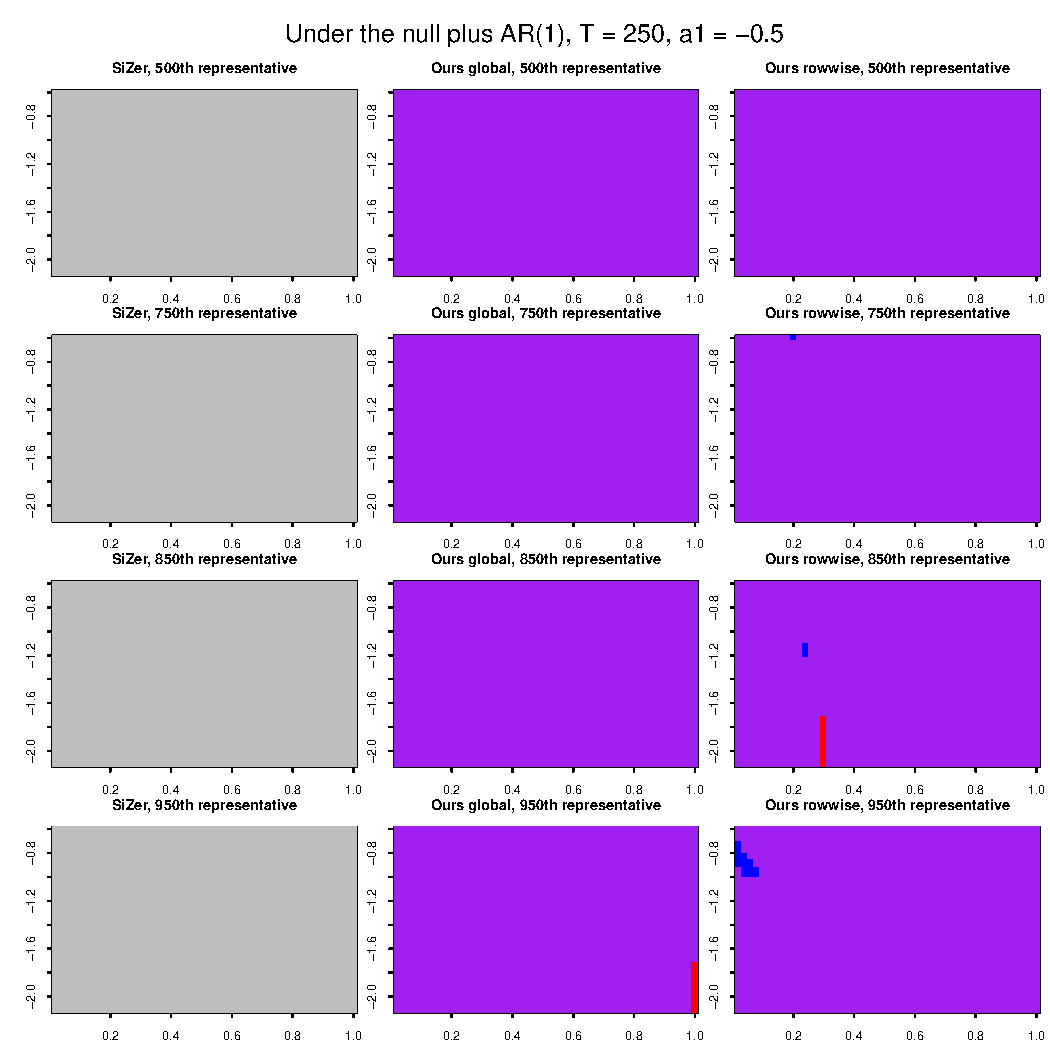
\includegraphics[width=\textwidth]{Plots/representatives_T_250_a1_-50_slope_0.pdf}
\caption{$a_1 = -0.5$}
\end{subfigure}\hspace{0.25cm}
\begin{subfigure}[b]{0.475\textwidth}
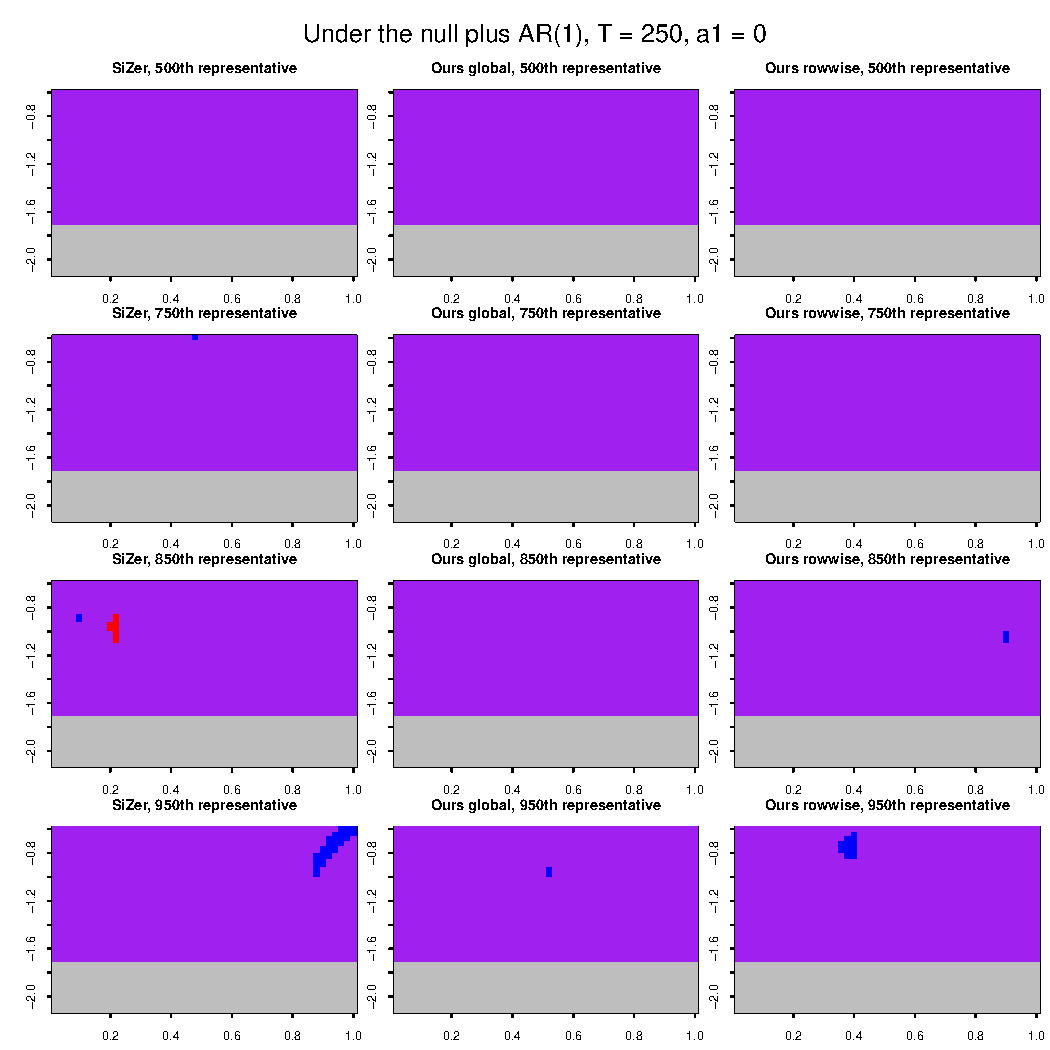
\includegraphics[width=\textwidth]{Plots/representatives_T_250_a1_0_slope_0.pdf}
\caption{$a_1 = 0$}
\end{subfigure}\\
\begin{subfigure}[b]{0.475\textwidth}
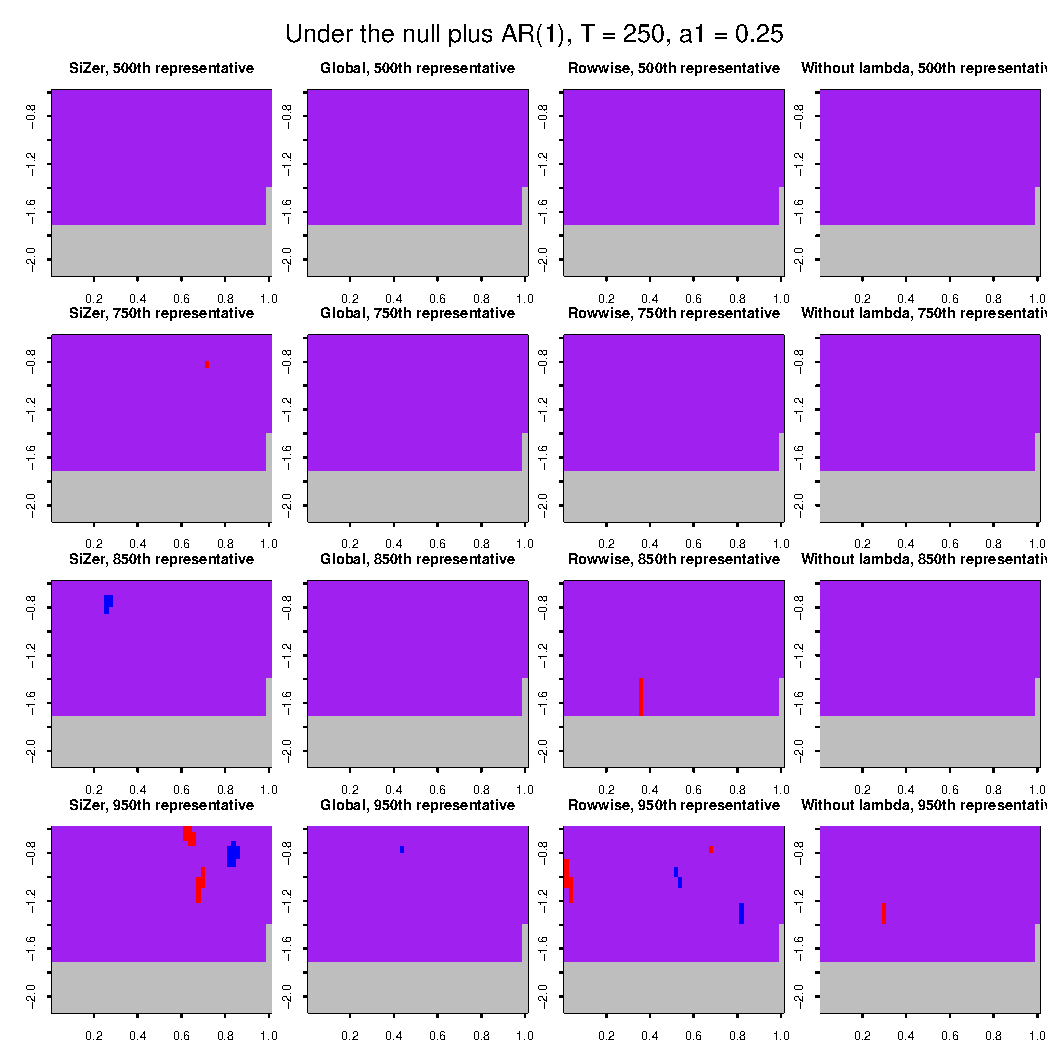
\includegraphics[width=\textwidth]{Plots/representatives_T_250_a1_25_slope_0.pdf}
\caption{$a_1 = 0.25$}
\end{subfigure}
\caption{Representative SiZer maps $T = 250$ and different AR(1) parameters $a_1 = -0.5, 0, 0.25$ in the simulation scenario under the null.}\label{fig:Representative_SiZer_maps}
\end{figure}


\bibliographystyle{ims}
{\small
\setlength{\bibsep}{0.55em}
\bibliography{bibliography}}


\end{document}
